\documentclass[12pt, a4paper]{article}
\usepackage[utf8]{inputenc} %usar acentuação em palavras
\usepackage[brazilian]{babel} %informar ao latex que o doc está sendo escrito em pt-br
\usepackage[T1]{fontenc} %copiar corretamente as palavras acentuadas no pdf
\usepackage{amsthm}
\usepackage{lipsum}
\usepackage[skip=-5pt]{caption} %colocar legendas em figuras
\captionsetup{font={stretch=0.6,small}} %fonte e tamanho das legendas

\usepackage{graphicx} %inserir figuras 
\usepackage{dsfont} %fonte para matemática



\theoremstyle{definition} %fonte das letras do exemplo e definição 
\newtheorem{defi}{Definição}[section]% apelido para chamar a definição e seccionar
\newtheorem{exem}{Exemplo}[section]


\title{\textbf{Definição de continuidade e limites de uma função vetorial em \LaTeX}}
\author{Eduardo Soares de Lima Filho
\\ \textbf{103146}}
\date{\today} %data atual do sistema

\begin{document}

	\maketitle %fazer o título 
	\newpage %folha nova
	
	\tableofcontents %criar sumário
	
	\newpage
	
	\section{Funções vetoriais \cite{livrocalc3}}
	
	\begin{defi}%1.1
	Uma função cujo domínio é o conjunto de números reais e cuja imagem é um conjunto de vetores é
	chamada função vetorial.
	\\
	Uma função vetorial definida em um intervalo $I \subset \mathds{R}$, com valores em $\mathds{R}^3$,
	é denotada por
	
	\begin{equation}
		\sigma(t) = (x(t), y(t), z(t)), t \in I
		\label{eq: 1}
	\end{equation}	 
	 
	
	
	O vetor $\sigma(t)$ é representado geometricamente pelo vetor $\stackrel{\longrightarrow}{OP}$, onde
	P = $(x(t),y(t),z(t))$; ver figura \ref{figura 1}
	
	\begin{center}
		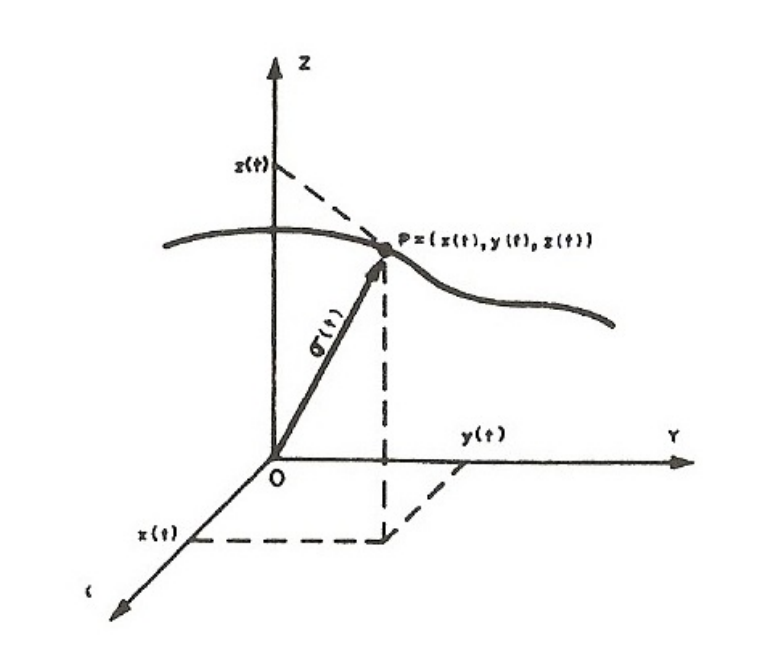
\includegraphics[width=0.5\textwidth]{grafico.png}
		\label{figura 1}
		\\ 
		\textbf{Figura 1.1} 
	\end{center}
	\end{defi}
	\\
	
	\begin{defi}\label{def1.2}%marcar para referenciar depois 
	O limite de $\sigma(t)$ quando $t$ se aproxima de $t_0$ é definido por 
	$$\lim_{t\to t_0}\sigma(t) = (\lim_{t\to t_0}x(t),\lim_{t\to t_0}y(t),
	\lim_{t\to t_0}z(t)),$$ 
	se $\lim\limits_{t\to t_0}x(t)$, $\lim\limits_{t\to t_0}y(t)$ e $\lim\limits_{t\to t_0}z(t)$ existem.
	\end{defi}	
	\\
	
	\begin{defi}\label{def1.3}
	A função $\sigma(t)$ é contínua em $t_0 \in I$ se, e somente se,
	$$\lim_{t \to t_0}\sigma(t) = \sigma(t_0).$$
	\\
	Segue das definições \ref{def1.2} e \ref{def1.3} que $\sigma(t)$ é contínua em $t_0$ se, e somente
	se, x(t), y(t) e z(t) são contínuas em $t_0$.
	\\
	\\
	Dizemos que a função $\sigma(t)$ \textbf{é contínua em I} se $\sigma(t)$ é contínua $\forall t 
	\in I.$
	\\
	\\
	Quando $\sigma(t)$ é contínua em $I$, o ponto final do vetor $\sigma(t) = (x(t),y(t),z(t))$ descreve 
	uma \textbf{curva C} no $\mathds{R}^3$, ou seja, para cada $t \in 	I$, obtemos um ponto 
	P = $(x,y,z)
	 \in$ C, onde
	 
	\begin{equation}
	x = x(t), \; y = y(t) \; e \;z = z(t).
	\label{eq: 2}
	\end{equation}
	\\
	A equação \ref{eq: 1} é dita uma \textbf{parametrização} da curva C, as equações \ref{eq: 2} são
	chamadas \textbf{equações paramétricas} da curva C e a variável t é o  \textbf{parâmetro}.
	\\
	Se eleminarmos o parâmetro t nas equações \ref{eq: 2}	 obteremos uma expressão cartesiana da curva
	C.
	
	 \end{defi}

	\begin{defi}\label{def1.4}
	A derivada da função vetorial $\sigma(t)$ com $t \in I= D_f \subset \mathds{R}$, é definida por  
	$$\sigma'(t) = \lim_{\bigtriangleup t\to 0}\frac{\sigma(t + \bigtriangleup t) - \sigma(t)}
	{\bigtriangleup t},$$  
	se o limite existir nos pontos $t \in I$.
	\\	
	Assim, segue das definções \ref{def1.2} e \ref{def1.4} e da definição de derivada de uma função real
	que
	$$\sigma'(t)=(x'(t),y'(t),z'(t))$$
	se $x'(t)$, $y'(t)$ e $z'(t)$ existirem.
	Dizemos que a função vetorial $\sigma(t)$ é \textbf{diferenciável} em I se $\sigma'(t)$ existir 
	$\forall t \in I$.
	\end{defi}
	
	\newpage	
	\\
	\bibliography{bibliografia} %referencias bibliogŕaficas
	\textbf{OBS:} Os textos são do livro referenciado acima acom apenas algumas modificações e 
	transcrito para a linguagem \LaTeX.

	




\end{document}